\documentclass[10pt,nofootinbib]{revtex4}
\usepackage[nocap]{ctex}
\usepackage{amsmath,amssymb,amsfonts,mathrsfs,bm,dsfont}
\usepackage{enumerate}
\usepackage{enumitem} % Customize itemize, see https://ctan.org/tex-archive/macros/latex/contrib/enumitem/
\usepackage[all]{xy}
\usepackage[normalem]{ulem}	% delete line
\usepackage{graphics,color}
\usepackage{tikz}
	\usetikzlibrary{calc}
	\usetikzlibrary{decorations.markings}
	\usetikzlibrary{arrows}
	\usetikzlibrary{patterns}
	%\usetikzlibrary{shapes.callouts}
\tikzset{
    level/.style = {
        ultra thick,
        blue,
    },
    connect/.style = {
        dashed,
        red
    },
    label/.style = {
        text width=2cm
    }
}
\usepackage{pgfplots}
%\usepackage[citestyle=authortitle]{biblatex} % able to cite the title, author and year
%\usepackage{hyperref}
\usepackage{feynmp} % feymann diagram
\usepackage{extarrows}

\usepackage[normalem]{ulem} % 文字划掉(横),与 cite 兼容问题,见 https://tex.stackexchange.com/questions/98222/ulem-incompatibility-with-multiple-entries-in-cite



\def\checkmark{\tikz\fill[scale=0.4](0,.35) -- (.25,0) -- (1,.7) -- (.25,.15) -- cycle;}

\def\dyz{\begin{tikzpicture}
	\draw[blue,scale=0.4] (0,0) .. controls (1,2.8) and (2.8,1) .. (0,0) .. controls (-1,-2.8) and (-2.8,-1) .. (0,0);
	%\node[blue] at (-1,-1) {$d_{yz,\sigma}$};
\end{tikzpicture}}
\def\dxz{\begin{tikzpicture}
	\draw[green,scale=0.4] (0,0) .. controls (-1,2.8) and (-2.8,1) .. (0,0) .. controls (1,-2.8) and (2.8,-1) .. (0,0);
	%\node[green] at (-1,1) {$d_{xz,\sigma}$};
\end{tikzpicture}}
\def\dxy{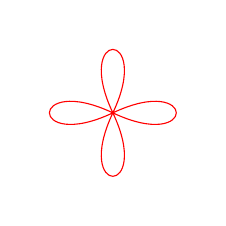
\begin{tikzpicture}
	\draw[red,scale=0.4,rotate=45] (0,0) .. controls (1,2.8) and (2.8,1) .. (0,0) .. controls (-1,-2.8) and (-2.8,-1) .. (0,0) .. controls (-1,2.8) and (-2.8,1) .. (0,0) .. controls (1,-2.8) and (2.8,-1) .. (0,0);
\end{tikzpicture}}

\def\oxy{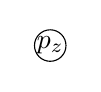
\begin{tikzpicture}
	\draw[fill=white,scale=0.4] (0,0) circle (0.5cm);
	\node at (0,0) {$p_z$};
\end{tikzpicture}}

\begin{document}
\title{Realization of Kitaev Model}
\author{Xiaodong Hu}
%\altaffiliation[Also at ]{Boson College}
\email{xiaodong.hu@bc.edu}
\affiliation{Department of Physics, Boston College}

\date{\today}

\begin{abstract}
	In this paper I will review the derivation of Kitaev coupling in honeycomb irridates. \par
	%\begin{center}
		\hfill\par
		{\centering\kaishu 谦谦君子,用涉大川。\par}
	%\end{center}
	\hfill------ 「易·谦卦」
\end{abstract}

\maketitle
\tableofcontents

\section{Effective Hilbert Space and Pseudospin}
	\subsection{Preliminaries: Crystal Field Splitting --- Representation of Octahedral Group $O_h$}
		In the cystal field of octahedral oxygen environment, the five $d$ orbitals of $\mathrm{Ir}$ atom (each of which can accommodate two electrons) will split into two-fold $e_g$ orbitals\footnote{Fundamentally, this result comes from the decomposition of the reducible five-dimensional representation of octahedral group (expressing in the basis of $d$ orbital wave function) \begin{equation*}
			\Gamma_d\equiv E\oplus T_2.
		\end{equation*}
		See \cite{sugano2012multiplets} and \cite{patrik1999lecture} for more details.}
		\begin{align*}
			|d_{x^2-y^2}\rangle&\equiv r^2(Y_2^2+Y_2^{-2}),\\
			|d_{3z^2-r^2}\rangle&\equiv r^2Y^0_2,
		\end{align*}
		and three-fold $t_{2g}$ orbitals
		\begin{align*}
			|d_{xz}\rangle&\equiv r^2(Y^1_2-Y_2^{-1}),\\
			|d_{yz}\rangle&\equiv r^2(Y^1_2+Y_2^{-1}),\\
			|d_{xy}\rangle&\equiv r^2(Y^2_2-Y_2^{-2}),
		\end{align*}
		as is illustrated in FIG. \ref{fig:1}. Further distortion, for example, Jahn-Teller effect, will split $t_{2g}$ orbitals into $a_{1g}$ and $e'_g$ as well, but we only truncate our discussion at the level of $t_{2g}$ orbitals.
		\begin{figure}[!htp]
			\centering
			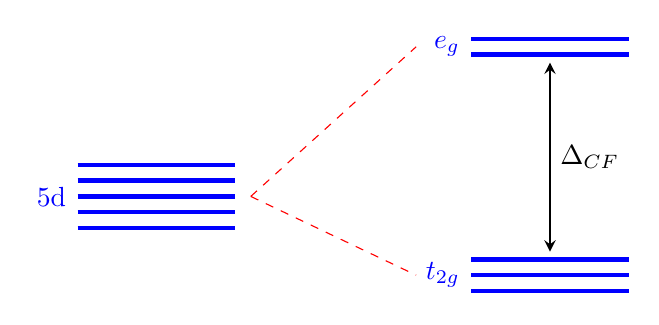
\begin{tikzpicture}
				% Draw all levels
				\draw[level] (0,0) -- (2,0);
				\draw[level] (0,-0.2) -- (2,-0.2);
				\draw[level] (0,-0.4) -- (2,-0.4);
				\draw[level] (0,0.2) -- (2,0.2);
				\draw[level] (0,0.4) -- (2,0.4);
				\draw[level] (0,0) node[left] {5d};

				\draw[connect] (2.2,0) -- (4.3,-1) (2.2,0) -- (4.3,1.9);
				
				\draw[level] (5,2) --  (7,2);
				\draw[level] (5,1.8) -- (7,1.8);
				\draw[level] (5,1.9) node[left] {$e_g$};

				\draw[level] (5,-0.8) -- (7,-0.8);
				\draw[level] (5,-1) -- (7,-1);
				\draw[level] (5,-1.2) -- (7,-1.2);
				\draw[level] (5,-1) node[left] {$t_{2g}$};

				\draw[<->,>=stealth,thick] (6,-0.7) -- node[right] {$\Delta_{CF}$} (6,1.7);
				% Draw labels
				%\node[label] at (3.5,-3) {Octahedral Crystal Fields};
			\end{tikzpicture}
			\caption{{\bf Multi-orbital Effect}: Octahedral Crystal Field Splitting.}
			\label{fig:1}
		\end{figure}
	\subsection{Quenching of Orbital Angular Momentum --- $t_{2g}$-$p$ Equivalence}

		It can be seen that \textbf{\color{red}the confining action of angular momentum operator $\bm{L}$ within the subspace of $t_{2g}$ has exactly the same matrix element of the action within the standard $p$-orbital or $l_{\text{eff}}=1$ basis \cite{patrik1999lecture}}. This phenomenon is called \emph{$t_{2g}$-$p$ equivalence}. More precisely, one can construct the $l_{\text{eff}}=1$ eigen states $|m\rangle$ ($m\equiv +1,0,-1$) with $t_{2g}$ orbitals $|\alpha\rangle$ ($\alpha\equiv d_{xz}, d_{xy}, d_{yz}$) by
		\begin{equation}
			|+1\rangle\equiv\dfrac{1}{\sqrt{2}}(|d_{xz}\rangle+i|d_{yz}\rangle),\quad|0\rangle\equiv|d_{xy}\rangle,\quad|-1\rangle\equiv\dfrac{1}{\sqrt{2}}(|d_{xz}\rangle-i|d_{yz}\rangle),
		\end{equation}
		and vice versa.	\textbf{We will work elaborately about the physical hopping of $d$-orbital electrons, both direct exchange of the Ir-Ir bond and indirect exchange of $\pi/2$ Ir-O-Ir bonds, so the unitary transformation between \emph{orbital representation} and \emph{angular momentum representation} is demanded}
		\begin{equation}\label{1.2.1}
			U_{\alpha m}\equiv\langle \alpha|m\rangle=\left(\begin{array}{ccc}
				1/\sqrt{2} & 0 & 1/\sqrt{2} \\
				0 & 1 & 0\\
				i/\sqrt{2} & 0 & -i/\sqrt{2}
			\end{array}\right).
		\end{equation}

	\subsection{$t_{2g}$ Splitting and Pseudospins from Spin-Orbital Coupling}
		It is believed that the $d$-orbital electron on each Ir atom experiences a \emph{strong} spin-orbital\footnote{Clearly the ``orbital momentum'' here is the effective one with $l_{\text{eff}}=1$.} coupling
		\begin{equation}\label{1.3.1}
			H_{\text{SOC}}=\lambda\bm{L\cdot S}+\Delta L_z^2\simeq \lambda\bm{L\cdot S}\equiv\dfrac{\lambda}{2}\left((\bm{L}+\bm{S})^2-\bm{L}^2-\bm{S}^2\right).
		\end{equation}
		\indent \textbf{We will show in this subsection that such SOC Hamiltonian split $t_{2g}$ orbitals further into $j_{\text{eff}}=1/2$ doublet subspace and $j_{\text{eff}}=3/2$ quadruplet subspace. So the low-energy effective spin (actually for the hole) is $1/2$}.\par
		In the (effective) $l$-$s$ representation $|ms\rangle\equiv(+1\uparrow,+1\downarrow,0\uparrow,0\downarrow,-1\uparrow,-1\downarrow)^T$, Hamiltonian \eqref{1.3.1} reads
		\begin{equation}\label{1.3.2}
			\varepsilon_{ls}\equiv\langle ms|H_{\text{SOC}}|ms\rangle=\left(\begin{array}{cccccc}
				\lambda/2 & 0 & 0 & 0 & 0 & 0\\
				0 & -\lambda/2 & \lambda/\sqrt{2} & 0 & 0 & 0\\
				0 & \lambda/\sqrt{2} & 0 & 0 & 0 & 0\\
				0 & 0 & 0 & 0 & \lambda/\sqrt{2} & 0\\
				0 & 0 & 0 & \lambda/\sqrt{2} & -\lambda/2 & 0\\
				0 & 0 & 0 & 0 & 0 & \lambda/2
			\end{array}\right).
		\end{equation}
		So under the basis of orbital representation $|\alpha s\rangle\equiv(d_{xz}\uparrow,d_{xz}\downarrow,d_{xy}\uparrow,d_{xy}\downarrow,d_{yz}\uparrow,d_{yz}\downarrow)^T$ we have
		\begin{equation*}
			\varepsilon_{\alpha s}\equiv\langle \alpha s|H_{\text{SOC}}|\alpha s\rangle=\sum_m\langle \alpha s|ms\rangle\langle ms|H_{\text{SOC}}|ms\rangle\langle ms|\alpha s\rangle.
		\end{equation*}
		Now that spin degree of freedoms are included, the unitary transformation \eqref{1.2.1} should also be enlarged to
		\begin{equation}\label{1.3.3}
			U\equiv U_{\alpha m}\otimes \sigma_0=
			\left(\begin{array}{cccccc}
				1/\sqrt{2} & 0 & 0 & 0 & 1/\sqrt{2} & 0 \\
				0 & 1/\sqrt{2} & 0 & 0 & 0 & 1/\sqrt{2} \\
				0 & 0 & 1 & 0 & 0 & 0 \\
				0 & 0 & 0 & 1 & 0 & 0 \\
				i/\sqrt{2} & 0 & 0 & 0 & -i/\sqrt{2} & 0 \\
				0 & i/\sqrt{2} & 0 & 0 & 0 & -i/\sqrt{2} \\
			\end{array}\right)
		\end{equation}
		Then
		\begin{equation}\label{1.3.4}
			\varepsilon_{\alpha s}=U \varepsilon_{ls} U^\dagger=
				\dfrac{\lambda}{2}\left(\begin{array}{cccccc}
					 0 & 0 & 0 & 1 & -i & 0 \\
					 0 & 0 & 1 & 0 & 0 & i \\
					 0 & 1 & 0 & 0 & 0 & -i \\
					 1 & 0 & 0 & 0 & i & 0 \\
					 i & 0 & 0 & -i & 0 & 0 \\
					 0 & -i & i & 0 & 0 & 0 \\
				\end{array}\right),
		\end{equation}
		which have two eigenvalues  $-\lambda$ and $\lambda/2$, indicating the further splitting of $t_{2g}$ orbitals to low energy doublet subspace and higher energy of quadruplet subspace.\par
		For the low-energy doublet subspace whose eigenvalue is $-\lambda$, the two-fold degenerate normalized eigen states, denoting as $|\widetilde{\uparrow}\rangle $ and $|\widetilde{\downarrow}\rangle $, are (note that we are now in the basis of $|\alpha s\rangle$)
		\begin{equation}\label{1.3.5}
			|\widetilde{\uparrow}\rangle=\dfrac{1}{\sqrt{3}}\bigg(|d_{xz}\downarrow\rangle-|d_{xy}\uparrow\rangle+|d_{yz}\downarrow\rangle\bigg),\quad|\widetilde{\downarrow}\rangle=\dfrac{1}{\sqrt{3}}\bigg(-|d_{xz}\uparrow\rangle-i|d_{xy}\downarrow\rangle+|d_{yz}\uparrow\rangle\bigg).
		\end{equation}
		That's why we say spin-orbital coupling leads to the emergence of pseudospin $j_{\text{eff}}=1/2$. And {\color{red}\textbf{the low-energy doublet subspace can be extracted from arbitrary form of Hamiltonian in use of the projection operator constructed from \eqref{1.3.5}}}
		\begin{equation}\label{1.3.6}
			P=\dfrac{1}{\sqrt{3}}\left(\begin{array}{cc}
				0 & i\\
				-i & 0\\
				i & 0\\
				0 & -i\\
				0 & 1\\
				1 & 0
			\end{array}\right).
		\end{equation}
		Particularly, one can check that
		\begin{equation*}
			P^\dagger \varepsilon_{\alpha s}P=\left(\begin{array}{cc}
				-\lambda & \\
				& -\lambda
			\end{array}\right) 
		\end{equation*}
\section{Hamiltonian}
	\subsection{On-site Hamiltonian}
		\subsubsection{Free Part}
			Introducing a six-component electron (hole) field\footnote{Note that the spin degree of freedoms on $d$-orbital electron field operators here are the pseudospin we introduced after consideration of spin-orbital-coupling induced splitting.} $d_i\equiv(d_{i,xz,\widetilde{\uparrow}},d_{i,xz,\widetilde{\downarrow}},d_{i,yz,\widetilde{\uparrow}},d_{i,yz,\widetilde{\downarrow}},d_{i,xy,\widetilde{\uparrow}},d_{i,xy,\widetilde{\downarrow}})^T$ on the $i$-th Ir atom, for a nearest neighbor Ir-Ir link (which is enough in our further description of hopping and interaction) the energy is simply the summation of on-site Hamiltonian
			\begin{equation}\label{2.1.1}
				H_0=d_1^\dagger \varepsilon_0 d_1+d_2^\dagger \varepsilon_0 d_2.
			\end{equation}
			But since  energy scale can be set to arbitrary value, we will ignore this trivial constant in the following discussion.
		
		\subsubsection{Coulomb Interaction Part}
			Except for the free part Hamiltonian, every electron (here is actually a hole) on the Ir site experiences strong (screened) Coulomb repulsive interaction (and we ignore the inter-site interaction for tight-binding approximation). So our next task is to express the second quantized two-body interaction on the $i$-th Ir atom
			\begin{align}\label{2.1.2}
				H_I&\equiv\dfrac{1}{2}\sum_{i\neq j}V(\bm{r}_i-\bm{r}_j)\equiv\dfrac{1}{2}\sum_{\substack{r_1,r_2,r_3,r_4\\\sigma_1,\sigma_2,\sigma_3,\sigma_4}}\langle\bm{r}_1,\sigma_1;\bm{r}_2,\sigma_2|V(\bm{r}_i-\bm{r}_j)\otimes\mathds{1}|\bm{r}_3,\sigma_3;\bm{r}_4,\sigma_4\rangle \psi_{\sigma_1}^\dagger(\bm{r}_1)\psi_{\sigma_2}^\dagger(\bm{r}_2)\psi_{\sigma_3}(\bm{r}_3)\psi_{\sigma_4}(\bm{r}_4)\nonumber\\
				&=\dfrac{1}{2}\sum_{\sigma,\sigma'}\int\mathrm{d}\bm{r}\,\mathrm{d}\bm{r'}\,\psi_\sigma^\dagger(\bm{r})\psi_{\sigma'}^\dagger(\bm{r'})V(\bm{r}-\bm{r'})\psi_{\sigma'}(\bm{r'})\psi_\sigma(\bm{r})
			\end{align}
			 in terms of the orbital momentum representation.\par
			 Expanding the position representation eigen states with $t_{2g}$ orbital states that
			 \begin{equation*}
			 	|\bm{r},\sigma\rangle\equiv\left(\sum_{\alpha\in\{xz,yz,xy\}}|\alpha\rangle\langle \alpha|\bm{r}\rangle\right)\otimes|\sigma\rangle\equiv\sum_\alpha\varphi_\alpha(\bm{r})|\alpha\rangle\otimes|\sigma\rangle\equiv\sum_\alpha\varphi_\alpha(\bm{r})|\alpha,\sigma\rangle,
			 \end{equation*}
			 then one immediately gets\footnote{In our convention of notation, $|\bm{r},\sigma\rangle\equiv \psi_\sigma(\bm{r})^\dagger|\Omega\rangle$ and $|\alpha,\sigma\rangle\equiv d_{\alpha,\sigma}^\dagger|\Omega\rangle$.}
			 \begin{equation}\label{2.1.3}
			 	H_I=\dfrac{1}{2}\sum_{\sigma,\sigma'}\sum_{\alpha_1,\alpha_2,\alpha_3,\alpha_4}d_{\alpha_1,\sigma}^\dagger d_{\alpha_2,\sigma'}^\dagger V_{\alpha_1,\alpha_2,\alpha_3,\alpha_4}d_{\alpha_3,\sigma'} d_{\alpha_4,\sigma},
			 \end{equation}
			 where
			 \begin{equation*}
			 	V_{\alpha_1,\alpha_2,\alpha_3,\alpha_4}\equiv \int\mathrm{d}\bm{r}\,\mathrm{d}\bm{r'}\,\varphi^*_{\alpha_1}(\bm{r})\varphi^*_{\alpha_2}(\bm{r'})V(\bm{r}-\bm{r'})\varphi_{\alpha_3}(\bm{r'})\varphi_{\alpha_4}(\bm{r}).
			 \end{equation*}
			{\color{red}Symmetry argument \cite{coury2016hubbard,castellani1978magnetic}} shows that
			\begin{equation}\label{2.1.4}
				V_{\alpha,\beta,\mu,\nu}\equiv U\delta_{\alpha \beta}\delta_{\mu \nu}\delta_{\alpha \mu}+V\delta_{\alpha\nu}\delta_{\beta\mu}(1-\delta_{\alpha \beta})+J\bigg(\delta_{\alpha \beta}\delta_{\mu\nu}(1-\delta_{\alpha\mu})+\delta_{\alpha\mu}\delta_{\beta\nu}(1-\delta_{\alpha\beta})\bigg),
			\end{equation}
			with $U\equiv V+2J$, where $U$ is the intra-orbital Hubbard interaction and $V$ is the inter-orbital direct interaction. The first term of $J$ is the Hund's rule exchange interaction, while the second term is the pair hopping interaction \cite{You-Kitaev}. Finally we have
			\begin{align}
				H_I&=\dfrac{U}{2}\sum_{\sigma,\sigma'}\sum_\alpha d_{\alpha,\sigma}^\dagger d_{\alpha,\sigma'}^\dagger d_{\alpha,\sigma'}d_{\alpha,\sigma}+\dfrac{V}{2}\sum_{\sigma,\sigma'}\sum_{\alpha\neq\beta} d_{\alpha,\sigma}^\dagger d_{\beta,\sigma'}^\dagger d_{\beta,\sigma'}d_{\alpha,\sigma}\nonumber\\
				&\qquad+\dfrac{J}{2}\sum_{\sigma,\sigma'}\sum_{\alpha\neq\beta}\left(d_{\alpha,\sigma}^\dagger d_{\beta,\sigma'}^\dagger d_{\alpha,\sigma'}d_{\beta,\sigma}+d_{\alpha,\sigma}^\dagger d_{\alpha,\sigma'}^\dagger d_{\beta,\sigma'}d_{\beta,\sigma}\right).\label{2.1.5}
			\end{align}
		
		\subsubsection{On-Site Two-Particle Hilbert Space}
			On each $i$-th site of Ir atom Coulomb interaction $H_I$ involves in two electrons (holes), so to combine all terms in Hamiltonian for further projection onto the correct low-energy sector, we have to enlarge the previous $6$-dimensional single-particle basis $\{d^\dagger_{\alpha,\sigma}|\Omega\rangle\}$ to two-particle one
			\begin{equation}\label{2.1.6}
				\mathcal{H}_{\text{intra-site}}\equiv \{d^\dagger_{i,\alpha,\sigma}d^\dagger_{i,\alpha',\sigma'}|\Omega\rangle\}.
			\end{equation}
			The dimensionality of this \emph{on-site} two-particle Hilbert space becomes $5+4+\cdots+1=15$ due to Pauli exclusion principle. More precisely, under the $15$-dimentional basis (for convenience labeled from $1$ to $15$)
			\begin{equation*}
				(\underbrace{d_{xz \widetilde{\uparrow} }^\dagger d_{xz \widetilde{\downarrow} }^\dagger,\cdots, d_{xz \widetilde{\uparrow} }^\dagger d_{xy \widetilde{\downarrow} }^\dagger}_{\text{5}};\underbrace{d_{xz \widetilde{\downarrow} }^\dagger d_{yz \widetilde{\uparrow} }^\dagger,\cdots,d_{xz \widetilde{\downarrow} }^\dagger d_{xy \widetilde{\downarrow} }^\dagger}_{\text{4}};\underbrace{d_{yz \widetilde{\uparrow} }^\dagger d_{yz \widetilde{\downarrow} }^\dagger,\cdots,d_{yz \widetilde{\uparrow} }^\dagger d_{xy \widetilde{\downarrow} }^\dagger}_{\text{3}};\underbrace{d_{yz \widetilde{\downarrow} }^\dagger d_{xy \widetilde{\uparrow} }^\dagger,d_{yz \widetilde{\downarrow} }^\dagger d_{xy \widetilde{\downarrow} }^\dagger}_{\text{2}};\underbrace{d_{xy \widetilde{\uparrow} }^\dagger d_{xy \widetilde{\downarrow} }^\dagger}_{\text{1}})^T|\Omega\rangle,
			\end{equation*}
			the matrix of $H_I$ in \eqref{2.1.5} takes the form of (after re-arrangement)
			\begin{equation}\label{2.1.7}
				H_I=\left(\begin{array}{ccccccccccccccc}
					 -U & 0 & 0 & 0 & 0 & 0 & 0 & 0 & 0 & -J & 0 & 0 & 0 & 0 & -J \\
					 0 & J-V & 0 & 0 & 0 & 0 & 0 & 0 & 0 & 0 & 0 & 0 & 0 & 0 & 0 \\
					 0 & 0 & -V & 0 & 0 & J & 0 & 0 & 0 & 0 & 0 & 0 & 0 & 0 & 0 \\
					 0 & 0 & 0 & J-V & 0 & 0 & 0 & 0 & 0 & 0 & 0 & 0 & 0 & 0 & 0 \\
					 0 & 0 & 0 & 0 & -V & 0 & 0 & J & 0 & 0 & 0 & 0 & 0 & 0 & 0 \\
					 0 & 0 & J & 0 & 0 & -V & 0 & 0 & 0 & 0 & 0 & 0 & 0 & 0 & 0 \\
					 0 & 0 & 0 & 0 & 0 & 0 & J-V & 0 & 0 & 0 & 0 & 0 & 0 & 0 & 0 \\
					 0 & 0 & 0 & 0 & J & 0 & 0 & -V & 0 & 0 & 0 & 0 & 0 & 0 & 0 \\
					 0 & 0 & 0 & 0 & 0 & 0 & 0 & 0 & J-V & 0 & 0 & 0 & 0 & 0 & 0 \\
					 -J & 0 & 0 & 0 & 0 & 0 & 0 & 0 & 0 & -U & 0 & 0 & 0 & 0 & -J \\
					 0 & 0 & 0 & 0 & 0 & 0 & 0 & 0 & 0 & 0 & J-V & 0 & 0 & 0 & 0 \\
					 0 & 0 & 0 & 0 & 0 & 0 & 0 & 0 & 0 & 0 & 0 & -V & J & 0 & 0 \\
					 0 & 0 & 0 & 0 & 0 & 0 & 0 & 0 & 0 & 0 & 0 & J & -V & 0 & 0 \\
					 0 & 0 & 0 & 0 & 0 & 0 & 0 & 0 & 0 & 0 & 0 & 0 & 0 & J-V & 0 \\
					 -J & 0 & 0 & 0 & 0 & 0 & 0 & 0 & 0 & -J & 0 & 0 & 0 & 0 & -U \\
				\end{array}\right).
			\end{equation}


	\subsection{Inter-Site Hamiltonian}
		\subsubsection{Hopping Part}
			For a general hopping (keeping the spin orientaion) on Ir-Ir link we have 
			\begin{equation}\label{2.2.1}
				H_t=d_1^\dagger T_{12} d_2+h.c.
			\end{equation}
			Following the supplementary material of \cite{rau2014generic}, since such Ir-Ir bond (as well as the surrounding octahedral oxygen atoms) possesses \emph{time-reversal symmetry} and \emph{inversion symmetry} about the bond center, we must have
			\begin{equation*}
				\rho(T)^\dagger H_t\rho(T)=d_1^\dagger T_{12}^* d_2+h.c.\equiv H_t\implies T_{12}^*\equiv T_{12}
			\end{equation*}
			 since representaion of time-reversal symmetry is anti-unitary and \emph{anti-linear}, and
			\begin{equation*}
				\rho(P)^\dagger H_t\rho(P)=d_2^\dagger T_{12} d_1+h.c.\equiv H_t\implies T_{12}\equiv T_{21}.
			\end{equation*}
			Therefore the hopping matrix $T_{12}$ must be \emph{real} and \emph{symmetric}
			\begin{equation*}
				T_{12}=\left(\begin{array}{ccc}
					T_{12}^{xz,xz} & T_{12}^{xz,yz} & T_{12}^{xz,xy} \\
					T_{12}^{xz,yz} & T_{12}^{yz,yz} & T_{12}^{yz,xy} \\
					T_{12}^{xz,xy} & T_{12}^{yz,xy} & T_{12}^{xy,xy} 
				\end{array}\right)\otimes \sigma_0.
			\end{equation*}
			\indent But this is not the end of the story. Along Ir-Ir bond direction, or $[110]$ direction in a local coordinate system, we also have a $C_2$ rotational symmetry such that $t_{2g}$ orbitals transform like $d_{xz,\sigma}\mapsto d_{yz,\sigma}$, $d_{yz,\sigma}\mapsto d_{xz,\sigma}$, and $d_{xy,\sigma}\mapsto d_{xy,\sigma}$. Therefore, hopping matrix $T_{12}$ takes the form of
			\begin{equation}\label{2.2.2}
				\rho(C_2)^\dagger H_t\rho(C_2)\equiv H_t\implies T_{12}=\left(\begin{array}{ccc}
					t_1 & t_2 & t_4 \\
					t_2 & t_1 & t_4 \\
					t_4 & t_4 & t_3
				\end{array}\right)\otimes\sigma_0.
			\end{equation}
			\indent Matrix \eqref{2.2.2} consists of both direct Ir-Ir exchange and indirect $\pi/2$ Ir-O-Ir exchange, as is shown in FIG. \ref{fig:direct} and FIG. \ref{fig:indirect}. Similar illustration can also be found in the recent analysis of $d^7$ cobalt compond in \cite{liu2018pseudospin} and \cite{sano2018kitaev}.\par
			\begin{figure}[!htp]
				\centering
				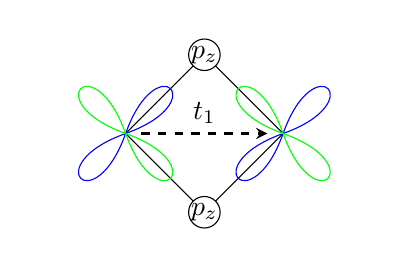
\begin{tikzpicture}
					\draw (0,0)--(1,1)--(2,0)--(1,-1)--cycle;
					\node at (0,0) {\dyz};
					\node at (0,0) {\dxz};
					\node at (2,0) {\dyz};
					\node at (2,0) {\dxz};					
					\node at (1,1) {\oxy};
					\node at (1,-1) {\oxy};
					\draw[->,>=stealth,thick,dashed] (0.2,0)--(1.8,0);
					\node[above] at (1,0) {$t_1$};
				\end{tikzpicture}
				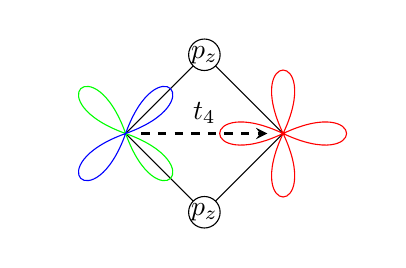
\begin{tikzpicture}
					\draw (0,0)--(1,1)--(2,0)--(1,-1)--cycle;
					\node at (0,0) {\dxz};
					\node at (0,0) {\dyz};
					\node at (2,0) {\dxy};
					\node at (1,-1) {\oxy};
					\node at (1,1) {\oxy};
					\draw[->,>=stealth,thick,dashed] (0.2,0)--(1.8,0);
					\node[above] at (1,0) {$t_4$};
				\end{tikzpicture}
				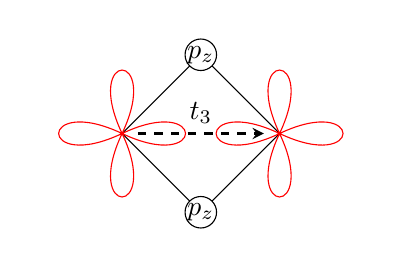
\begin{tikzpicture}
					\draw (0,0)--(1,1)--(2,0)--(1,-1)--cycle;
					\node at (0,0) {\dxy};
					\node at (2,0) {\dxy};
					\node at (1,1) {\oxy};
					\node at (1,-1) {\oxy};
					\draw[->,>=stealth,thick,dashed] (0.2,0)--(1.8,0);
					\node[above] at (1,0) {$t_3$};
				\end{tikzpicture}
				\caption{{\bf Direct Exchange between Ir-Ir Orbitals}. Blue one is the $t_{2g}$ orbital of $d_{yz,\sigma}$, red one is $d_{xy,\sigma}$, and green one is $d_{yz,\sigma}$.}
				\label{fig:direct}
			\end{figure}
			
			\begin{figure}[!htp]
				\centering
				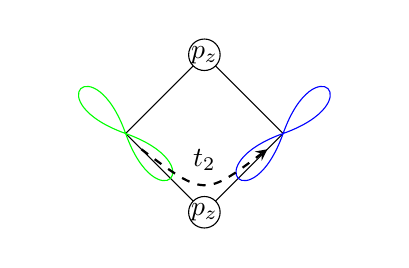
\begin{tikzpicture}
					\draw (0,0)--(1,1)--(2,0)--(1,-1)--cycle;
					\node at (0,0) {\dxz};
					\node at (2,0) {\dyz};
					\node at (1,1) {\oxy};
					\node at (1,-1) {\oxy};
					\draw[->,>=stealth,thick,dashed] (0.2,-0.2)..controls(1,-0.8)..(1.8,-0.2);
					\node[above] at (1,-0.6) {$t_2$};
				\end{tikzpicture}
				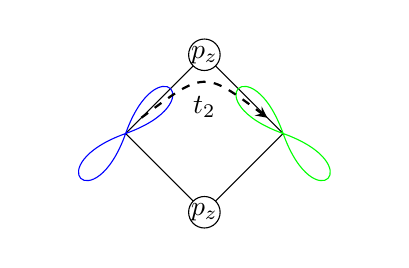
\begin{tikzpicture}
					\draw (0,0)--(1,1)--(2,0)--(1,-1)--cycle;
					\node at (0,0) {\dyz};
					\node at (2,0) {\dxz};
					\node at (1,1) {\oxy};
					\node at (1,-1) {\oxy};
					\draw[->,>=stealth,thick,dashed] (0.2,0.2)..controls(1,0.8)..(1.8,0.2);
					\node[below] at (1,0.6) {$t_2$};
				\end{tikzpicture}
				\caption{{\bf Hopping Mediated by Oxygen $p$-Orbitals}.}
				\label{fig:indirect}
			\end{figure}
			Detailed physical meanings of hopping matrix elements relating to so-called \emph{Slater-Koster} parameter \cite{slater1954simplified} are given in the supplementary material of \cite{rau2014generic}.

		\subsubsection{Inter-Site Two-Particle Hilbert Space}
			Similar to the \emph{quartic} form of Coulomb term we encountered before, where \emph{on-site} two-particle Hilbert space is demanded for accommodation of the matrix elements, since the \emph{quadratic} hopping Hamiltonian $H_t$ involves two electrons (holes) on \emph{distinct} sites of Ir atoms this time, we still have to consider the two-particle Hilbert space to accommodate the hopping matrix elements, while Pauli exclusion principle is quenched this time. So the dimensionality of out new \emph{inter-site} two-particle basis, (taking the hopping processes from site $2$ to site $1$ as an example)
			\begin{equation}\label{2.2.3}
				\mathcal{H}_{\text{inter-site}}=\{(d_1)_{\alpha,\sigma}^\dagger(d_2)_{\alpha',\sigma'}|\Omega\rangle\}
			\end{equation}
			is $6\times 6=36$. And hopping matrix under \eqref{2.2.3} takes the form of
			\begin{equation}\label{2.2.4}
				T=\mathds{1}\otimes T_{12}+T_{21}\otimes\mathds{1},
			\end{equation}
			where $\mathds{1}$ is a $6$-dimensional identity matrix on the opposite transition sector.\par
			Let us focus on the site-$1$ physics. Hopping matrix $d_1^\dagger T_{12}d_2$ will transfer electrons (holes) from site $2$ to site $1$, formally resulting in a new \emph{$36$-dimensional on-site} two-particle basis
			\begin{equation*}
				\widetilde{\mathcal{H}}_{\text{on-site}} \equiv d_1^\dagger T_{12}d_2(\mathcal{H}_{\text{inter-site}})=\{(d_1)_{\alpha,\sigma}^\dagger(d_1)_{\alpha',\sigma'}|\Omega\rangle\}.
			\end{equation*}

			\noindent But as is mentioned above, because of the existence of Pauli exclusion principle, not all hopping channels are physically allowed. In fact, real physical hoppings occur only on the $15$-dimensional \emph{on-site} two-particle Hilbert space $\mathcal{H}_{\text{on-site}}$ we constructed in the previous section instead of $\widetilde{\mathcal{H}}_{\text{on-site}}$. To achieve this, again we need a projection
			\begin{equation}\label{2.2.5}
				\mathcal{P}_t\widetilde{\mathcal{H}}_{\text{on-site}}=\mathcal{H}_{\text{on-site}},
			\end{equation}
			where $\mathcal{P}_t$ is a $15\times36$ matrix
			\begin{equation*}
				\mathcal{P}_t^T=\left(
				\begin{array}{ccccccccccccccc}
					0 & 0 & 0 & 0 & 0 & 0 & 0 & 0 & 0 & 0 & 0 & 0 & 0 & 0 & 0 \\
					1 & 0 & 0 & 0 & 0 & 0 & 0 & 0 & 0 & 0 & 0 & 0 & 0 & 0 & 0 \\
					0 & 1 & 0 & 0 & 0 & 0 & 0 & 0 & 0 & 0 & 0 & 0 & 0 & 0 & 0 \\
					0 & 0 & 1 & 0 & 0 & 0 & 0 & 0 & 0 & 0 & 0 & 0 & 0 & 0 & 0 \\
					0 & 0 & 0 & 1 & 0 & 0 & 0 & 0 & 0 & 0 & 0 & 0 & 0 & 0 & 0 \\
					0 & 0 & 0 & 0 & 1 & 0 & 0 & 0 & 0 & 0 & 0 & 0 & 0 & 0 & 0 \\
					-1 & 0 & 0 & 0 & 0 & 0 & 0 & 0 & 0 & 0 & 0 & 0 & 0 & 0 & 0 \\
					0 & 0 & 0 & 0 & 0 & 0 & 0 & 0 & 0 & 0 & 0 & 0 & 0 & 0 & 0 \\
					0 & 0 & 0 & 0 & 0 & 1 & 0 & 0 & 0 & 0 & 0 & 0 & 0 & 0 & 0 \\
					0 & 0 & 0 & 0 & 0 & 0 & 1 & 0 & 0 & 0 & 0 & 0 & 0 & 0 & 0 \\
					0 & 0 & 0 & 0 & 0 & 0 & 0 & 1 & 0 & 0 & 0 & 0 & 0 & 0 & 0 \\
					0 & 0 & 0 & 0 & 0 & 0 & 0 & 0 & 1 & 0 & 0 & 0 & 0 & 0 & 0 \\
					0 & -1 & 0 & 0 & 0 & 0 & 0 & 0 & 0 & 0 & 0 & 0 & 0 & 0 & 0 \\
					0 & 0 & 0 & 0 & 0 & -1 & 0 & 0 & 0 & 0 & 0 & 0 & 0 & 0 & 0 \\
					0 & 0 & 0 & 0 & 0 & 0 & 0 & 0 & 0 & 0 & 0 & 0 & 0 & 0 & 0 \\
					0 & 0 & 0 & 0 & 0 & 0 & 0 & 0 & 0 & 1 & 0 & 0 & 0 & 0 & 0 \\
					0 & 0 & 0 & 0 & 0 & 0 & 0 & 0 & 0 & 0 & 1 & 0 & 0 & 0 & 0 \\
					0 & 0 & 0 & 0 & 0 & 0 & 0 & 0 & 0 & 0 & 0 & 1 & 0 & 0 & 0 \\
					0 & 0 & -1 & 0 & 0 & 0 & 0 & 0 & 0 & 0 & 0 & 0 & 0 & 0 & 0 \\
					0 & 0 & 0 & 0 & 0 & 0 & -1 & 0 & 0 & 0 & 0 & 0 & 0 & 0 & 0 \\
					0 & 0 & 0 & 0 & 0 & 0 & 0 & 0 & 0 & -1 & 0 & 0 & 0 & 0 & 0 \\
					0 & 0 & 0 & 0 & 0 & 0 & 0 & 0 & 0 & 0 & 0 & 0 & 0 & 0 & 0 \\
					0 & 0 & 0 & 0 & 0 & 0 & 0 & 0 & 0 & 0 & 0 & 0 & 1 & 0 & 0 \\
					0 & 0 & 0 & 0 & 0 & 0 & 0 & 0 & 0 & 0 & 0 & 0 & 0 & 1 & 0 \\
					0 & 0 & 0 & -1 & 0 & 0 & 0 & 0 & 0 & 0 & 0 & 0 & 0 & 0 & 0 \\
					0 & 0 & 0 & 0 & 0 & 0 & 0 & -1 & 0 & 0 & 0 & 0 & 0 & 0 & 0 \\
					0 & 0 & 0 & 0 & 0 & 0 & 0 & 0 & 0 & 0 & -1 & 0 & 0 & 0 & 0 \\
					0 & 0 & 0 & 0 & 0 & 0 & 0 & 0 & 0 & 0 & 0 & 0 & -1 & 0 & 0 \\
					0 & 0 & 0 & 0 & 0 & 0 & 0 & 0 & 0 & 0 & 0 & 0 & 0 & 0 & 0 \\
					0 & 0 & 0 & 0 & 0 & 0 & 0 & 0 & 0 & 0 & 0 & 0 & 0 & 0 & 1 \\
					0 & 0 & 0 & 0 & -1 & 0 & 0 & 0 & 0 & 0 & 0 & 0 & 0 & 0 & 0 \\
					0 & 0 & 0 & 0 & 0 & 0 & 0 & 0 & -1 & 0 & 0 & 0 & 0 & 0 & 0 \\
					0 & 0 & 0 & 0 & 0 & 0 & 0 & 0 & 0 & 0 & 0 & -1 & 0 & 0 & 0 \\
					0 & 0 & 0 & 0 & 0 & 0 & 0 & 0 & 0 & 0 & 0 & 0 & 0 & -1 & 0 \\
					0 & 0 & 0 & 0 & 0 & 0 & 0 & 0 & 0 & 0 & 0 & 0 & 0 & 0 & -1 \\
					0 & 0 & 0 & 0 & 0 & 0 & 0 & 0 & 0 & 0 & 0 & 0 & 0 & 0 & 0
				\end{array}\right).
			\end{equation*}

\section{Large-U Approximation}
		
	\subsection{Self-Energy Operator}

	\subsection{Projection to Low-Energy Pseudospin Subspace}

	\subsection{Kitaev Coupling}
		\begin{figure}[!htp]
			\centering
			\includegraphics[scale=0.36]{Na2IrO3_Polyhedral.png}
			\caption{{\bf caption}:}
			\label{fig:Na2IrO3}
		\end{figure}
		
\bibliography{hxd}
\bibliographystyle{apsrev} % apsrev is format for PRL of APS
\end{document}